\documentclass[14pt,aspectratio=2013]{beamer}
\title{An Example of MOCK: The Simple Pendulum}
\author{Adam Handwerger}
\date{}
\usetheme{default}
\usepackage{amsmath,amsfonts,amssymb}
\usepackage{natbib}
\usepackage{booktabs}
\usepackage{stmaryrd}
\usepackage{nopageno}
\usepackage{hyperref}
\usepackage{bookmark}
\usepackage{mathtools}
\usepackage{pdfpages}
\usepackage{geometry}
\usepackage{relsize}
\usepackage{graphicx}
\usepackage{xfrac}
\usepackage{dsfont}
\usepackage{tikz}
\usepackage{tikz} \usetikzlibrary{angles,quotes}
\usepackage{relsize}
\usepackage{caption}
%\usepackage[style=apa]{biblatex}
\usepackage[utf8]{inputenc}
\begin{document}
\frame{\titlepage}
\begin{frame}
\vspace{1cm}   
\begin{center}
    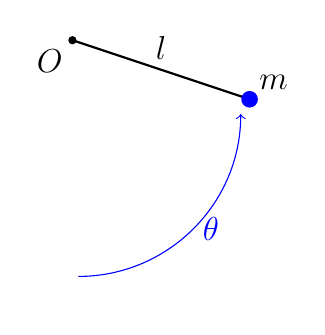
\begin{tikzpicture}[scale=.75]
    
        \tikzstyle{every node}=[font=\large]

        \draw [thick] -- (0, -3.5) -- (0, -4.5);
    
        % Define pivot point
        \coordinate (pivot) at (0,0);

        % Define bob position based on angle theta
        \coordinate (bob) at (3,-1);
        % Change (3,1) to adjust the length and the angle theta

        % Draw the pivot point
        \fill[black] (pivot) circle (2pt);

        % Draw the string
        \draw [thick] (pivot) -- (bob);

        % Draw the bob
        \fill[blue] (bob) circle (4pt);

        % Add angle label (theta)
        \draw[->, blue] (.1,-4.0) arc (-90:0:2.75) node[midway, right, blue] {$\theta$};
        % Adjust the radius and angle as desired.
        % Add labels for components
        \node[below left] at (pivot) {${O}$};
        \node[above right] at (bob) {${m}$};
        \node[right] at (0.5,0) {};
        \node[below] at (0, -1) {};
        \node[above] at (1.5,-0.5) {${l}$};
    \end{tikzpicture}
\end{center}   
\vspace{1cm}
\[
    \ddot{\theta}+\left(\dfrac{g}{l}\right)\sin(\theta)=0
\]
\end{frame}

\begin{frame}{State Space Representation}
    With $x(t)=[ \theta(t), \dot{\theta}(t) ]^{\top} \text{,   }\omega_0=\sqrt{\dfrac{g}{l}}$\\
    \vspace{1cm}

\begin{equation}
    \begin{bmatrix}
        \dot{x_1}(t) \\
        \dot{x_2}(t)
    \end{bmatrix}=
    \begin{bmatrix}
        x_2(t) \\
        -\omega_0^2 \sin{x_1(t)}
    \end{bmatrix} \tag{SS}
\end{equation}

\end{frame}

\begin{frame}{The Analytical Solution}
\vspace{.5cm}
The special function $\operatorname{sn}$ used below is called the Jacobi elliptic function.\\
\vspace{.5cm}
\[
    \theta(t)=2 \sin^{-1} \left(sin\frac{\theta_0}{2}sn \left[K\left(sin^2 \frac{\theta_0}{2}\right)-\omega_0t;sin^2 \frac{\theta_0}{2}\right]\right)
\]
    with\\
\[
    K(m)=\int\limits_0^1\dfrac{dz}{\sqrt{(1-z^2)(1-mz^2)}}
\]
\end{frame}

\begin{frame}{For small $\theta_0$ the pendulum is a harmonic oscillator}

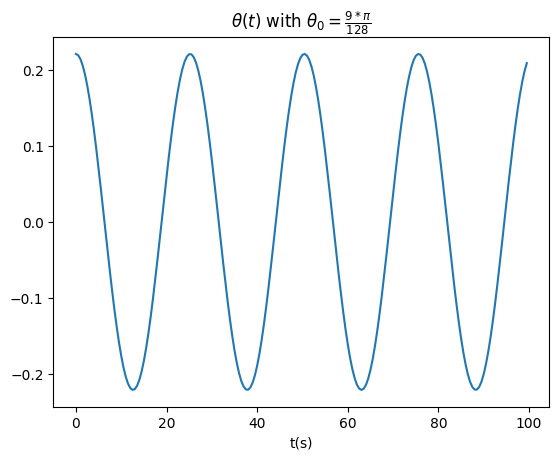
\includegraphics[scale=.6]{Projectplot_analytical.png}

\end{frame}

\begin{frame}{Synthesizing data for the MOCK training set}
The state space system (SS) was numerical integrated\\
to find $x(t)$ with solve\_ivp, using the DOP853 method.\\
From this, $\dot{\theta}$(t) was used along with the analytical\\
value $\theta(t)$
\end{frame}
\begin{frame}{Initial Values}
The various trajectories, $\theta_i(t)$ correspond to different $\theta_0$.\\
 For sythesizing the data a uniform distribution of intital positions
from $\theta_0=0 \text{ to } \theta_0=\frac{127}{128} \pi$ were used. Only \\
trajectories with zero intial velocity were considered.\\
\end{frame}
\begin{frame}{Accuracy of Numerical Integration}
The percent error is defined as $\dfrac{\parallel \theta_n(t)-\theta_a(t) \parallel}{\parallel \theta_a(t) \parallel}$x100\\
where $\theta_a(t)$ is the analytic solution and $\theta_n(t)$ is the numerical solution.
\end{frame}
\begin{frame}{Sample Trajectory from Validation Set}
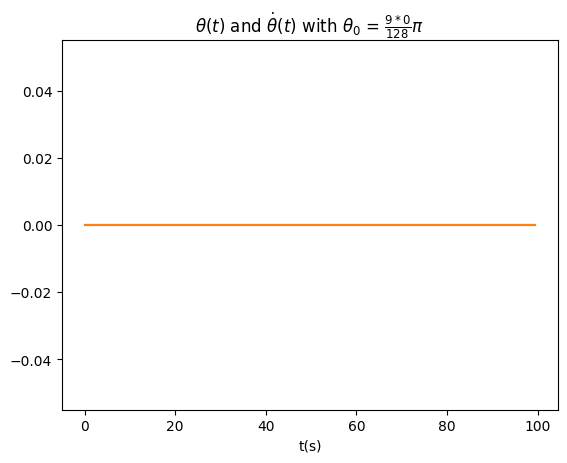
\includegraphics[scale=.5]{projectplot_trajectory0.png}\\
percent error=0.00
\end{frame}
\begin{frame}{Sample Trajectory from Validation Set}
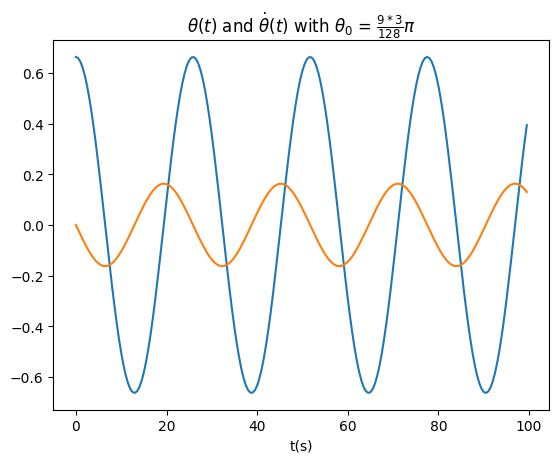
\includegraphics[scale=.5]{projectplot_trajectory3.png}\\
percent error=0.0018
\end{frame}
\begin{frame}{Sample Trajectory from Validation Set}
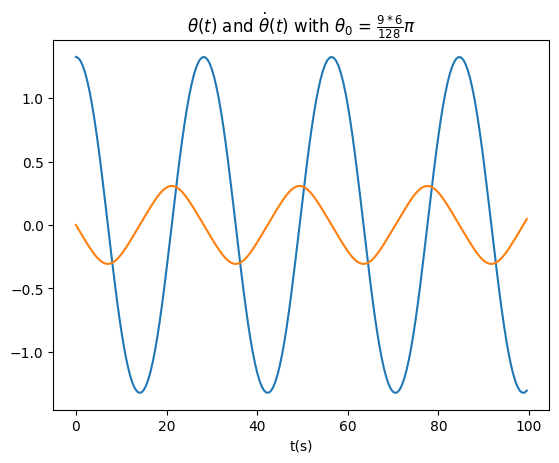
\includegraphics[scale=.5]{projectplot_trajectory6.png}\\
percent error=0.0010
\end{frame}
\begin{frame}{Sample Trajectory from Validation Set}
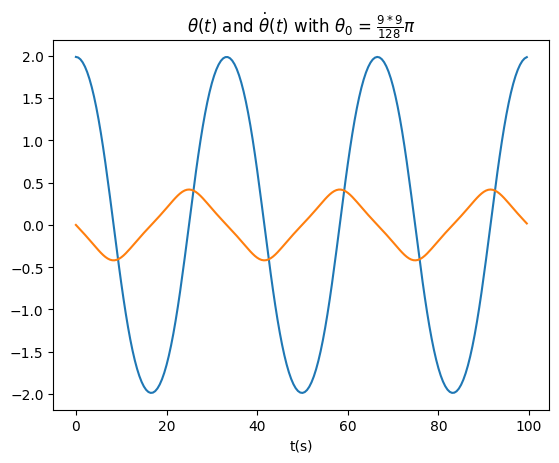
\includegraphics[scale=.5]{projectplot_trajectory9.png}\\
percent error=0.00092
\end{frame}
\begin{frame}{Sample Trajectory from Validation Set}
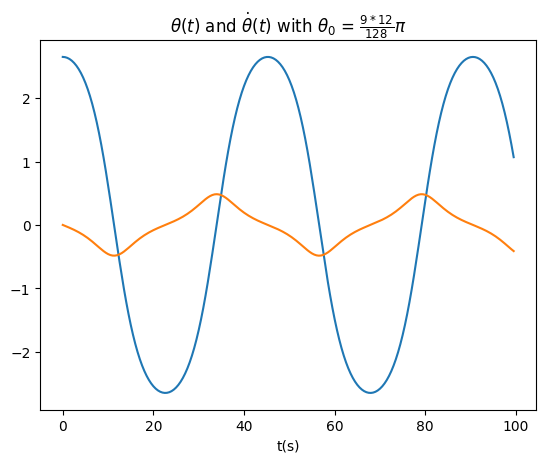
\includegraphics[scale=.5]{projectplot_trajectory12.png}\\
percent error=0.0019
\end{frame}
\begin{frame}{Sample Trajectory from Validation Set}
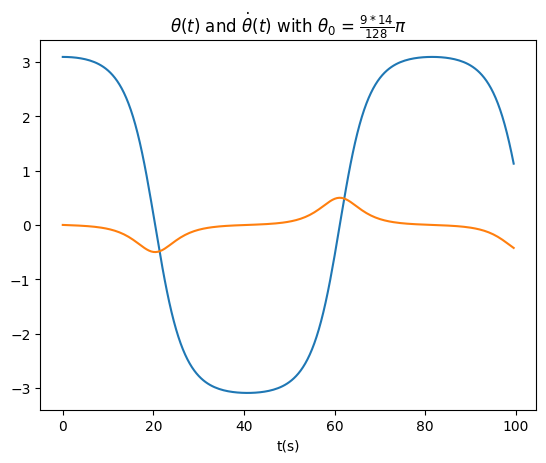
\includegraphics[scale=.5]{projectplot_trajectory14.png}\\
percent error=0.073
\end{frame}
\begin{frame}{Tuning the Hyperparameters $\gamma,\lambda$ with the Validation Set}
For the validation set we choose\\
\vspace{.5cm}
$\theta_0=\dfrac{9\pi*n}{128} \text{  for } n=0,1,...,14$\\
\vspace{.5cm}
which gave $\gamma=10 \text{ and } \lambda=5*10^{-7}$ as optimal.\\
\end{frame}
\begin{frame}{Slope Field of Sample Trajectories from Validation Set}
\begin{columns}[c]
     \begin{column}{.5\textwidth}
    \begin{figure}
        \centering
        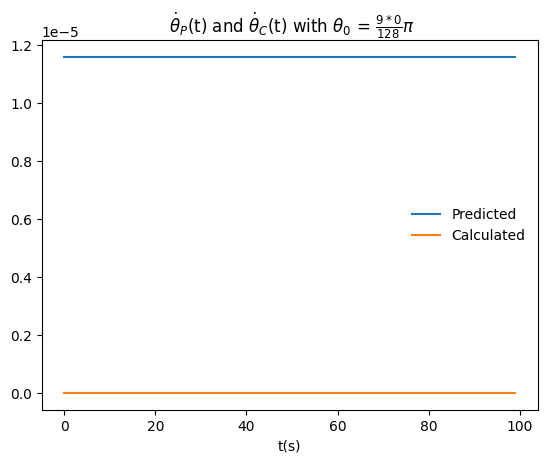
\includegraphics[width=.8\textwidth]{projectplot_thetadot0}
    \end{figure}
    \end{column}
        \begin{column}{.5\textwidth}
        \begin{figure}
        \centering
        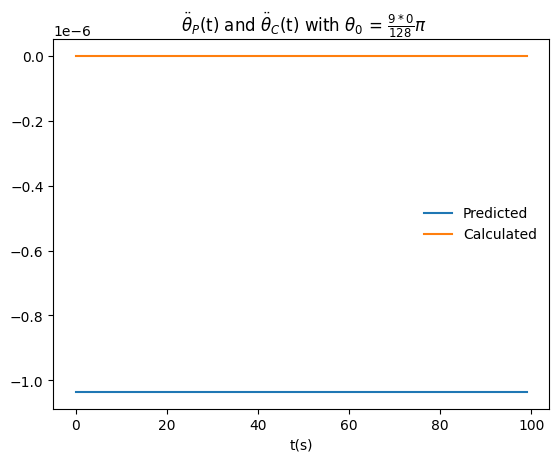
\includegraphics[width=.8\textwidth]{projectplot_thetadoubledot0} 
    \end{figure}
    \end{column}
\end{columns}
\end{frame}
\begin{frame}{Slope Field of Sample Trajectories from Validation Set}
    \begin{columns}[c]
         \begin{column}{.5\textwidth}
        \begin{figure}
            \centering
            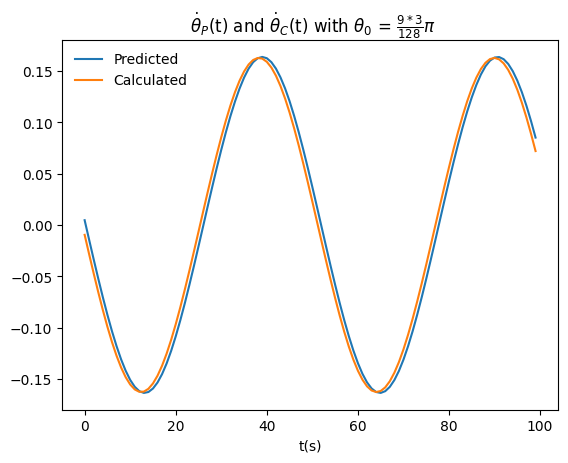
\includegraphics[width=.8\textwidth]{projectplot_thetadot3}
        \end{figure}
        \end{column}
            \begin{column}{.5\textwidth}
            \begin{figure}
            \centering
            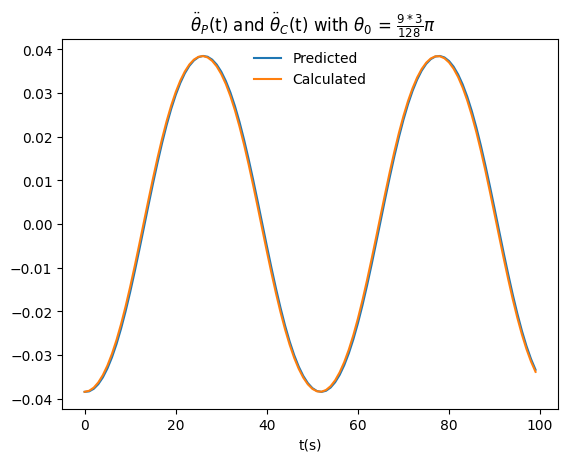
\includegraphics[width=.8\textwidth]{projectplot_thetadoubledot3} 
        \end{figure}
        \end{column}
    \end{columns}
    \end{frame}
\begin{frame}{Slope Field of Sample Trajectories from Validation Set}
    \begin{columns}[c]
        \begin{column}{.5\textwidth}
            \begin{figure}
            \centering
            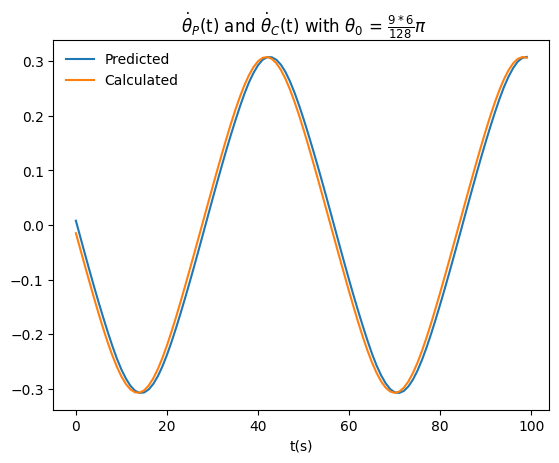
\includegraphics[width=.8\textwidth]{projectplot_thetadot6}
            \end{figure}
        \end{column}
        \begin{column}{.5\textwidth}
            \begin{figure}
            \centering
            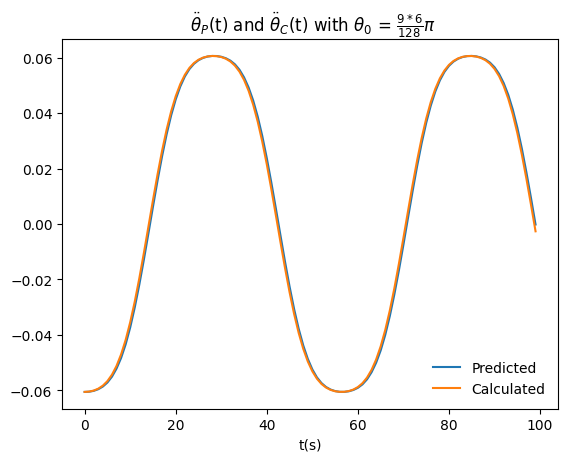
\includegraphics[width=.8\textwidth]{projectplot_thetadoubledot6} 
            \end{figure}
        \end{column}
        \end{columns}
\end{frame}
\begin{frame}{Slope Field of Sample Trajectories from Validation Set}
    \begin{columns}[c]
        \begin{column}{.5\textwidth}
        \begin{figure}
            \centering
            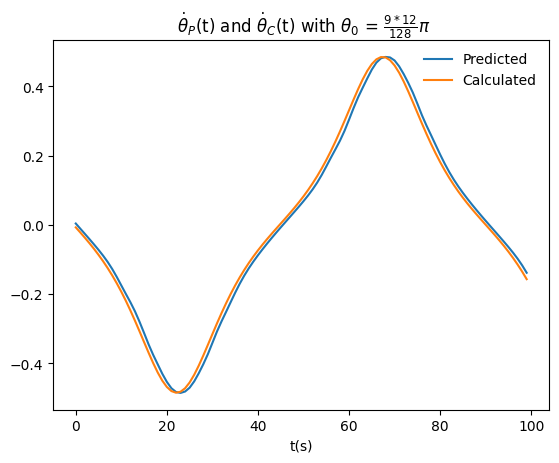
\includegraphics[width=.8\textwidth]{projectplot_thetadot9}
            \end{figure}
        \end{column}
        \begin{column}{.5\textwidth}
            \begin{figure}
            \centering
            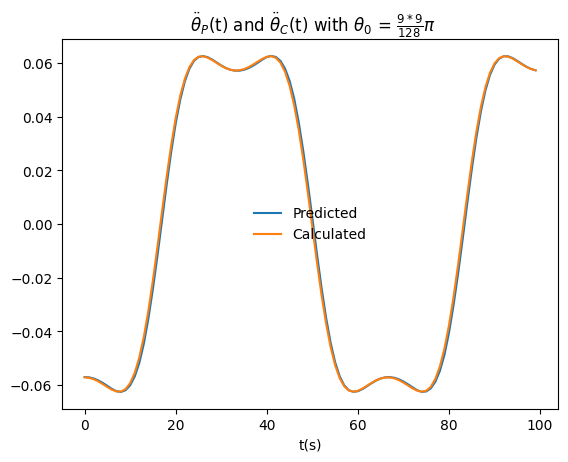
\includegraphics[width=.8\textwidth]{projectplot_thetadoubledot9} 
            \end{figure}
        \end{column}
    \end{columns}
\end{frame}
\begin{frame}{Slope Field of Sample Trajectories from Validation Set}
    \begin{columns}[c]
            \begin{column}{.5\textwidth}
                \begin{figure}
                \centering
                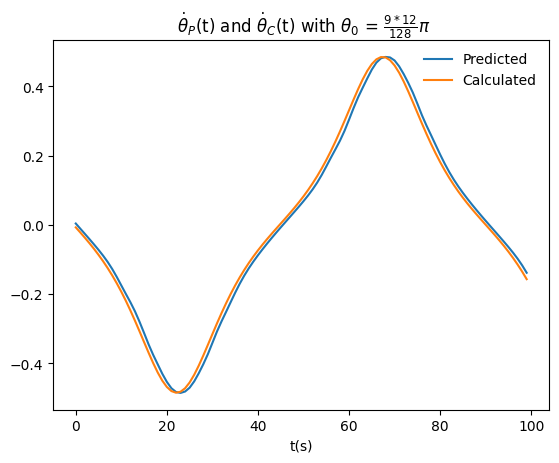
\includegraphics[width=.8\textwidth]{projectplot_thetadot12}
                \end{figure}
            \end{column}
            \begin{column}{.5\textwidth}
                \begin{figure}
                \centering
                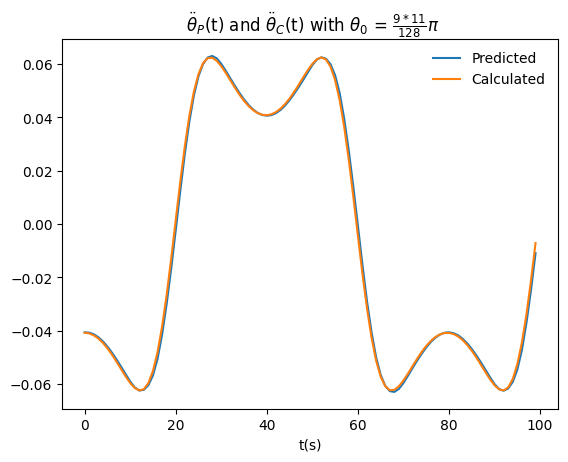
\includegraphics[width=.8\textwidth]{projectplot_thetadoubledot12} 
                \end{figure}
            \end{column}
        \end{columns}
\end{frame}
\begin{frame}{Slope Field of Sample Trajectories from Validation Set}
    \begin{columns}[c]
         \begin{column}{.5\textwidth}
            \begin{figure}
            \centering
            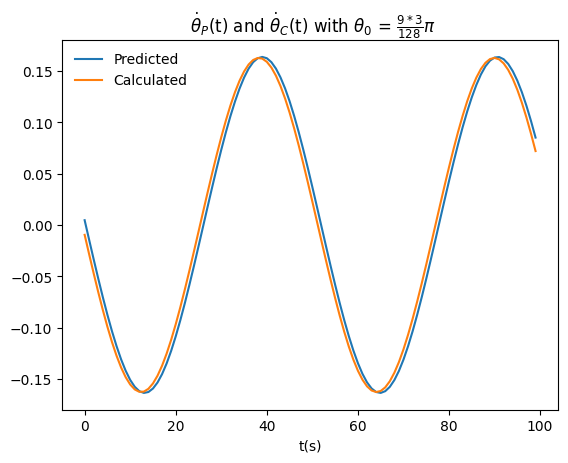
\includegraphics[width=.8\textwidth]{projectplot_thetadot3}
            \end{figure}
        \end{column}
        \begin{column}{.5\textwidth}
            \begin{figure}
            \centering
            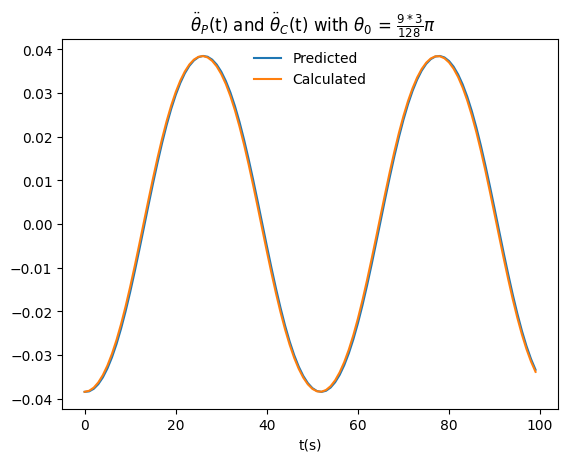
\includegraphics[width=.8\textwidth]{projectplot_thetadoubledot3} 
            \end{figure}
        \end{column}
    \end{columns}
    \end{frame}
    \begin{frame}{Slope Field of Sample Trajectories from Validation Set}
        \begin{columns}[c]
             \begin{column}{.5\textwidth}
                \begin{figure}
                \centering
                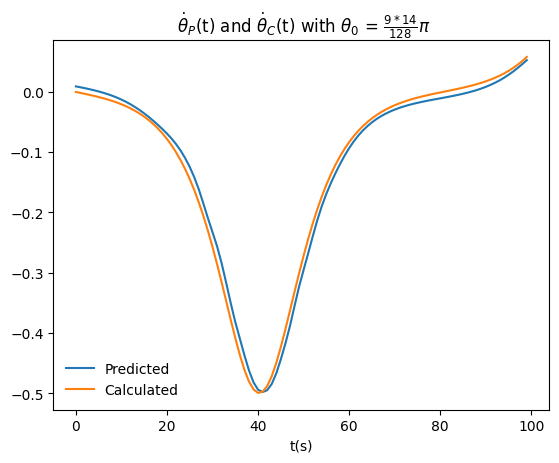
\includegraphics[width=.8\textwidth]{projectplot_thetadot14}
            \end{figure}
            \end{column}
                \begin{column}{.5\textwidth}
                \begin{figure}
                \centering
                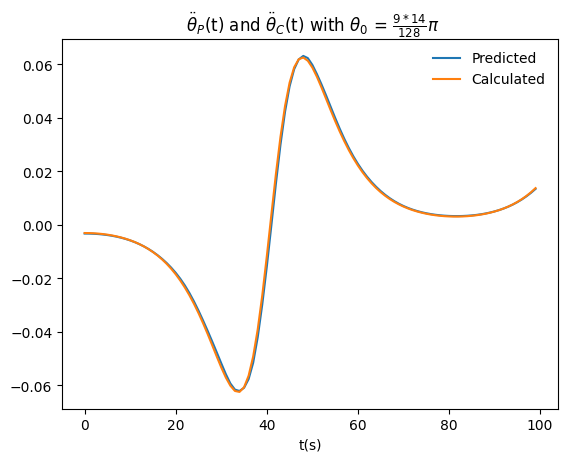
\includegraphics[width=.8\textwidth]{projectplot_thetadoubledot14} 
            \end{figure}
            \end{column}
        \end{columns}
    \end{frame}
     \begin{frame}{Slope Field of Sample Trajectories from Validation Set}
        \begin{columns}[c]
             \begin{column}{.5\textwidth}
                \begin{figure}
                \centering
                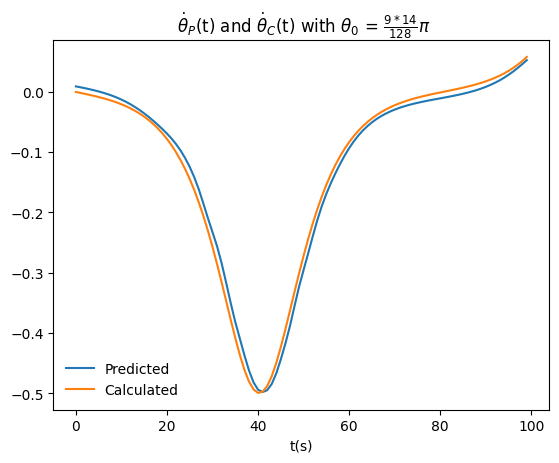
\includegraphics[width=.8\textwidth]{projectplot_thetadot14}
            \end{figure}
            \end{column}
                \begin{column}{.5\textwidth}
                \begin{figure}
                \centering
                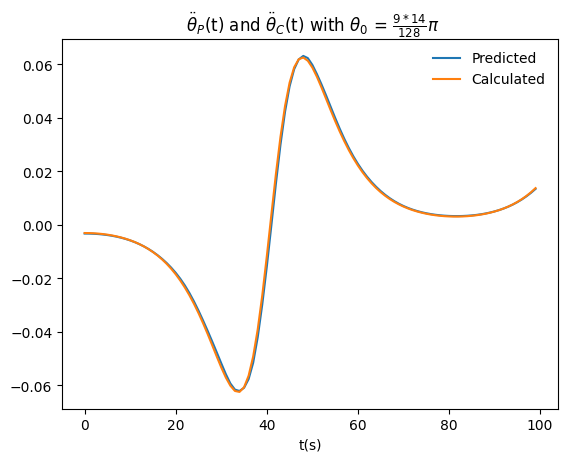
\includegraphics[width=.8\textwidth]{projectplot_thetadoubledot14} 
            \end{figure}
            \end{column}
        \end{columns}
    \end{frame}
     

\begin{frame}{The Training Set}
The training set consisted of 15 trajectories which were\\
slightly different from the validation set. The values of\\
$\theta_0$ were evenly spaced and ranged from $.0007 \pi$ to $0.985 \pi$.\\
\end{frame}

\begin{frame}{A Comparision of Trajectories as Predicted by MOCK vs. Analytical Derived}
The slope field derived by the MOCK method was\\
numerically integrated using the 'RK45' method for five\\
random trajectors with $\theta_0 \in (0,\pi)$ and compared\\
with more advanced methods available from the $solve\_ipv$\\
package. No noticable difference was seen in the results\\
by switching integration methods.
\end{frame}

\begin{frame}{A Comparision of Trajectories}
    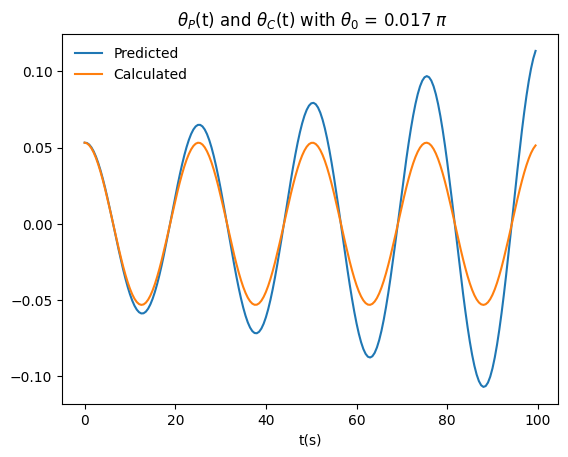
\includegraphics[scale=.5]{projectplot_result1}
\end{frame}
\begin{frame}{A Comparision of Trajectories}
    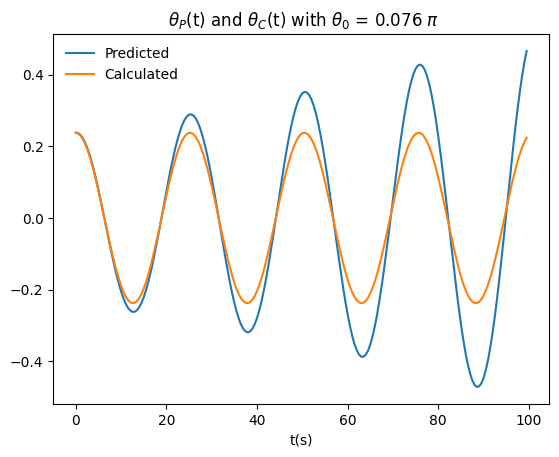
\includegraphics[scale=.5]{projectplot_result2}
\end{frame}
\begin{frame}{A Comparision of Trajectories}
    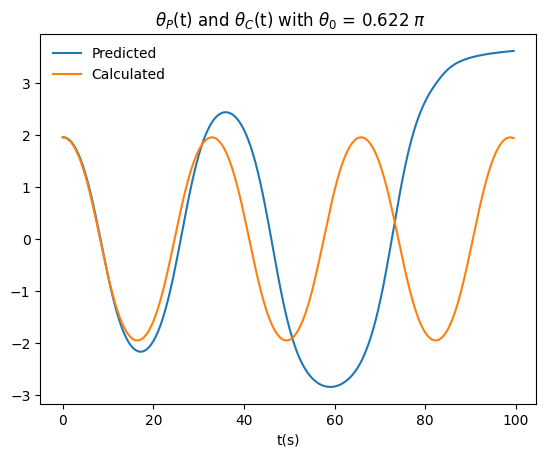
\includegraphics[scale=.5]{projectplot_result3}
\end{frame}
\begin{frame}{A Comparision of Trajectories}
    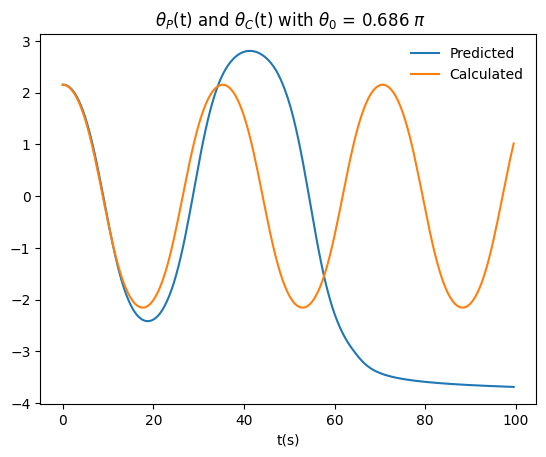
\includegraphics[scale=.5]{projectplot_result4}
\end{frame}
\begin{frame}{A Comparision of Trajectories}
    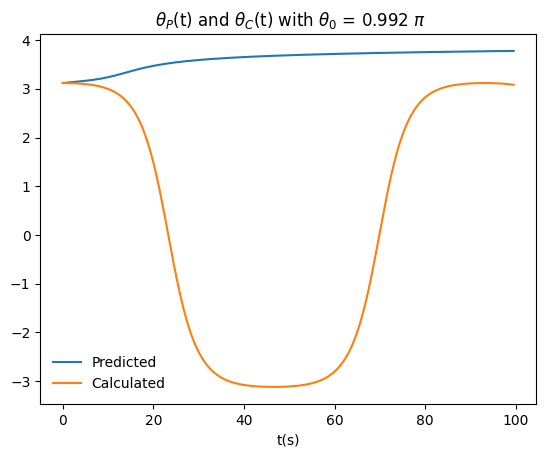
\includegraphics[scale=.5]{projectplot_result5}
\end{frame}
\begin{frame}{Possible Improvements to Modeling Trajectories}
    \begin{itemize}
        \item Add more trajectories to the training set
        \item Increase the sampling rate for each trajectory in the training set
    \end{itemize}
\end{frame}

\begin{frame}{Results}
Doublng the number of trajectories did not help with\\
learning the training set nor with $\theta_0$ chosen at random.\\
Doubling of the sampling rate lead to a substainal\\
improvement as shown below. This suggests that any\\
pendulum trajectory can be predicted for all time, \\
but only if the training set is sampled continuously.\\
\end{frame}
\begin{frame}{A Comparision of Different Sampling Rates}
    \begin{columns}[c]
         \begin{column}{.5\textwidth}
            \begin{figure}
            \centering
            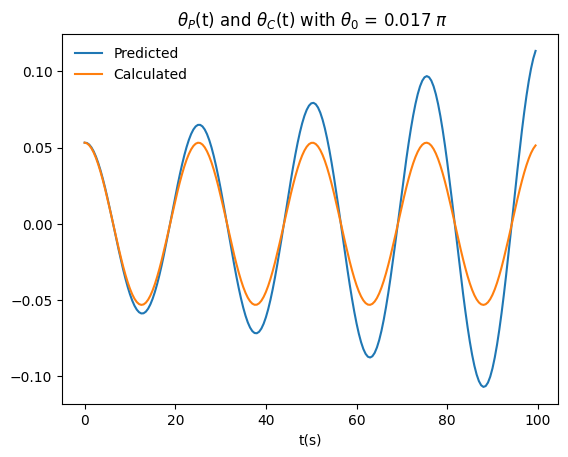
\includegraphics[width=.8\textwidth]{projectplot_result1}
        \end{figure}
        \end{column}
            \begin{column}{.5\textwidth}
            \begin{figure}
            \centering
            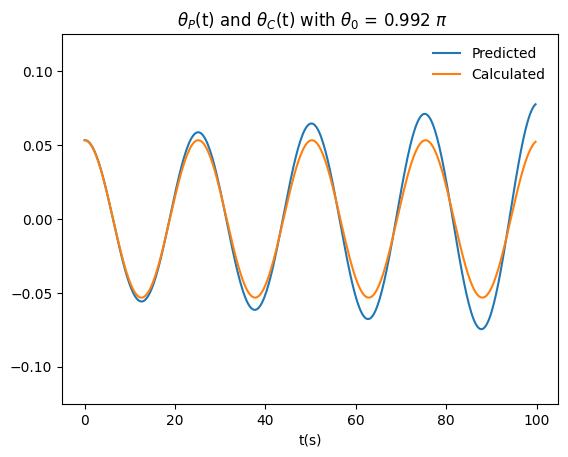
\includegraphics[width=.8\textwidth]{projectplot_resultprime1} 
        \end{figure}
        \end{column}
    \end{columns}
\end{frame}

\begin{frame}{A Comparision of Different Sampling Rates}
    \begin{columns}[c]
         \begin{column}{.5\textwidth}
            \begin{figure}
            \centering
            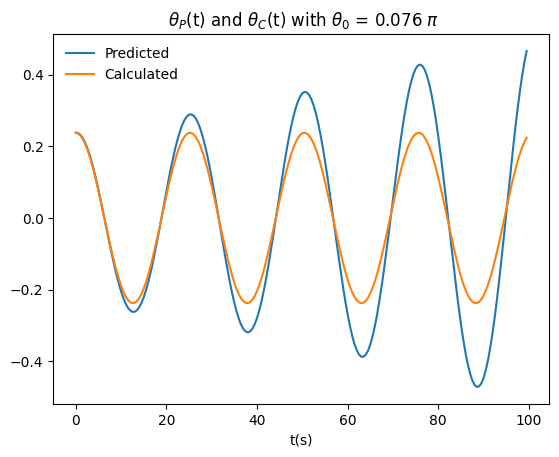
\includegraphics[width=.8\textwidth]{projectplot_result2}
        \end{figure}
        \end{column}
            \begin{column}{.5\textwidth}
            \begin{figure}
            \centering
            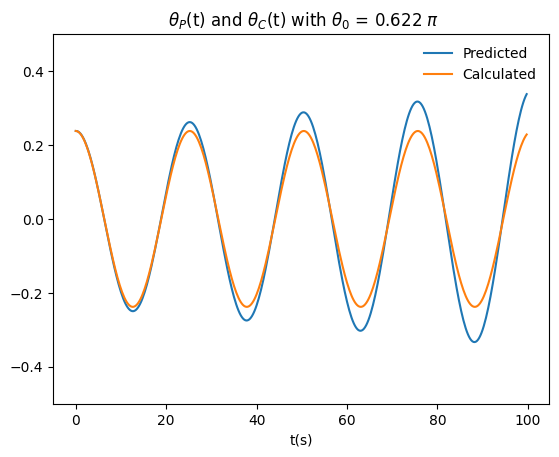
\includegraphics[width=.8\textwidth]{projectplot_resultprime2} 
        \end{figure}
        \end{column}
    \end{columns}
\end{frame}
\begin{frame}{A Comparision of Different Sampling Rates}
    \begin{columns}[c]
         \begin{column}{.5\textwidth}
            \begin{figure}
            \centering
            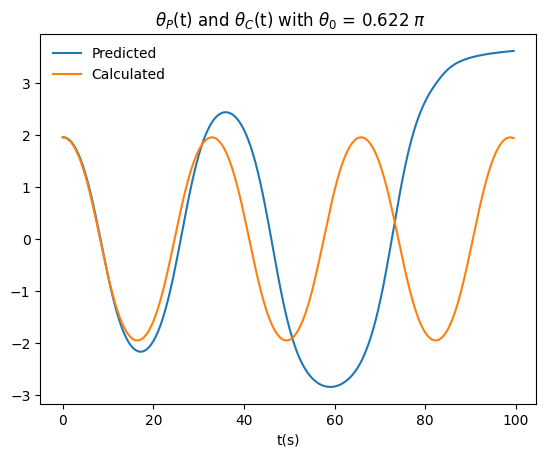
\includegraphics[width=.8\textwidth]{projectplot_result3}
        \end{figure}
        \end{column}
            \begin{column}{.5\textwidth}
            \begin{figure}
            \centering
            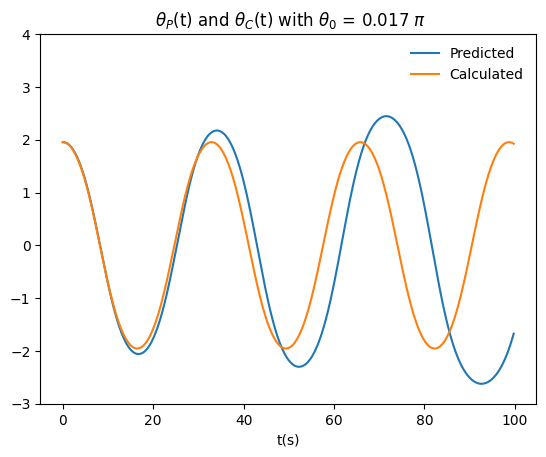
\includegraphics[width=.8\textwidth]{projectplot_resultprime3} 
        \end{figure}
        \end{column}
    \end{columns}
\end{frame}
\begin{frame}{A Comparision of Different Sampling Rates}
    \begin{columns}[c]
         \begin{column}{.5\textwidth}
            \begin{figure}
            \centering
            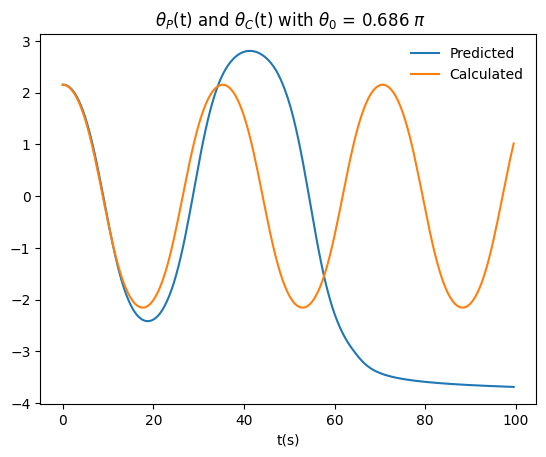
\includegraphics[width=.8\textwidth]{projectplot_result4}
        \end{figure}
        \end{column}
            \begin{column}{.5\textwidth}
            \begin{figure}
            \centering
            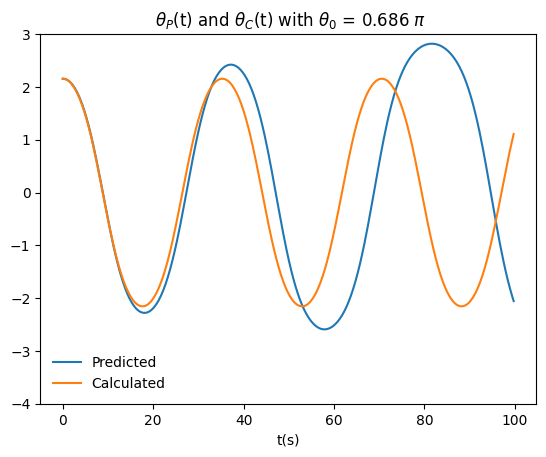
\includegraphics[width=.8\textwidth]{projectplot_resultprime4} 
        \end{figure}
        \end{column}
    \end{columns}
\end{frame}
\begin{frame}{A Comparision of Different Sampling Rates}
    \begin{columns}[c]
         \begin{column}{.5\textwidth}
            \begin{figure}
            \centering
            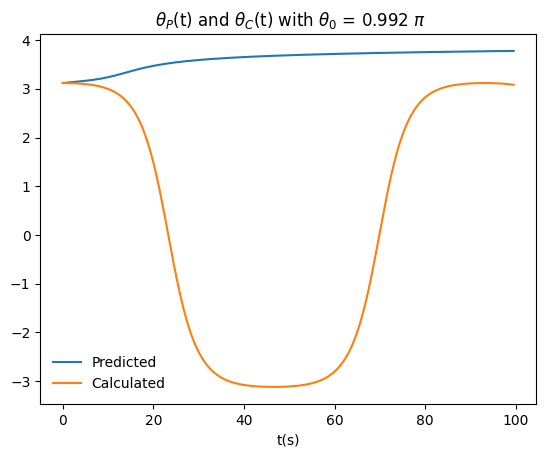
\includegraphics[width=.8\textwidth]{projectplot_result5}
        \end{figure}
        \end{column}
            \begin{column}{.5\textwidth}
            \begin{figure}
            \centering
            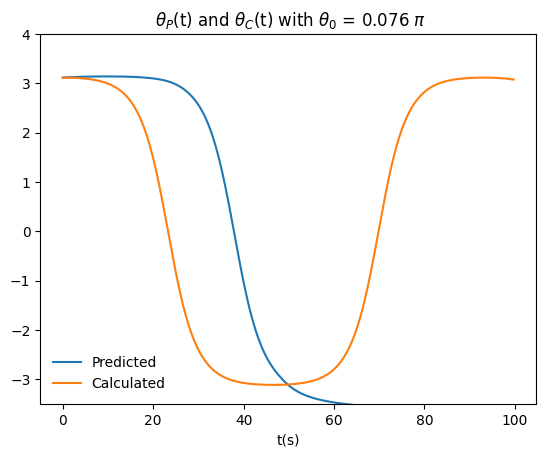
\includegraphics[width=.8\textwidth]{projectplot_resultprime5} 
        \end{figure}
        \end{column}
    \end{columns}
\end{frame}
\begin{frame}{References}
        (1) Rielly, V. et. all (2025, Jane 8) \emph{MOCK: an Algorithm}\\
        \emph{for Learning Nonparametric Differential Equations via}\\
        \emph{Multivariate Occupation Kernel Functions}, arXiv:2306.10189v3\\
        \vspace{1cm}
        (2) Bel\'endez,C. et. all (2007, Aug. 28) \emph{Exact solution}\\
        \emph{for the nonlinear pendulum,} Sociedade Brasileira de\\
        F\'isica, v. 29 n.4 p.645-648\\
\end{frame}

\end{document}